%!TEX root = ../../thesis.tex
%*******************************************************************************
%****************************** Background Chapter *********************************
%*******************************************************************************

\chapter{Background}
\ifpdf
    \graphicspath{{Chapters/Background/Figs/}{Chapters/Background/Figs/}{Chapters/Background/Figs/}}
\else
    \graphicspath{{Chapters/Background/Figs/}{Chapters/Background/Figs/}}
\fi
To build the foundation of our approach, we present the usage of crowdsourcing in software development (see section \ref{background:section:crowdsourcing}), UI Prototyping (see section \ref{background:section:uiprototyping}), Low and No code (see section \ref{background:section:lowcode}), Model Based Software Engineering (MBSE) (see section \ref{background:section:mbse}), Task Based Usability Testing (see section \ref{background:section:task}), and Experimental Product Design and define Design Principles (DP) (see section \ref{background:section:experimentproduct}).
%********************************** % Crowdsourcing of Software Products **************************************
\section{Crowdsourcing of Software Products}
\label{background:section:crowdsourcing}
Iterative feedback from potential customers can help improve the development of software products \cite{article:lean:eric}.
To do that, we can use crowdsourcing.
Crowdsourcing refers to outsourcing value-creating activities from a company by an open call to a large, undefined group of users to get feedback \cite{article:crowdsourcing:leimeister}.
The word crowdsourcing is a combination of crowd and outsourcing.
Crowdsourcing often involves less specialized and more generalized groups of participants than outsourcing \cite{article:crowdsourcing:estelles}.
Some advantages of crowdsourcing include lowered costs, improved speed, quality, flexibility, and scalability \cite{article:crowdsourcing:prpic}.
Researchers have used crowdsourcing in many research approaches, including \textit{crowd testing, crowd funding, crowd ideation, crowd logistic, crowd production, crowd promotion,} and \textit{crowd support} over the last few years \cite{article:crowdsourcing:durward}.
In our approach to finding a solution, we focus more on crowd-testing and crowd-ideation.

\paragraph{Crowd Testing:}
The companies use crowd-testing to evaluate different running software products with the users.
A growing trend in software testing is crowd testing, which utilizes the benefits, effectiveness, and efficiency of crowdsourcing and cloud platforms \cite{article:crowdsourcing:latoza}.
Crowd testing is considered when the software is more user-centric: i.e., software with a broad user base whose success is evaluated by user input.
CrowdStudy \cite{article:crowdsourcing:nebeling} is a method that enables developers to assess the usability of their web interfaces using crowd workers from Amazon Mechanical Turk\footnote{Amazon Mechanical Turk: \url{https://www.mturk.com}}.
CrowdCrit \cite{article:crowdsourcing:luther} is another tool that uses Amazon Mechanical Turk to support designers in validating created posters in the form of uploaded images.
Similarly, \textit{Interactive event-flow graphs} and \textit{GUI-level (Graphical User Interface) guidance} \cite{article:crowdsourcing:chen} are the two techniques to increase crowd testers' coverage for GUI using crowd-testing.

\paragraph{Crowd Ideation:}
Design can be infused with creativity by online crowds, but using traditional strategies to harness them, such as large-scale ideation platforms, requires organization and time \cite{article:crowdsourcing:andolina}.
Hence, crowd ideation is used to build new and improved versions of existing software product ideas with the consumers.
Under manipulations of task complexity, idea representation, and procedural guidance, Shixuan Fu et al. \cite{article:crowdsourcing:fu} examine how cognitive load is altered during idea generation and convergence with crowds.
ERICA \cite{article:crowdsourcing:erica} is a tool that uses expert knowledge to validate diverse crowd answers.
Crowdboard \cite{article:crowdsourcing:andolina} is a tool used to engage crowds in real-time brainstorming, concept mapping, and other design processes at an early stage of the design process.
There were, however, no approaches that directly addressed prototype application areas.

%********************************** % UI Prototyping **************************************
\clearpage
\section{UI Prototyping}
\label{background:section:uiprototyping}
\begin{figure}[htbp!]
  \centering    
  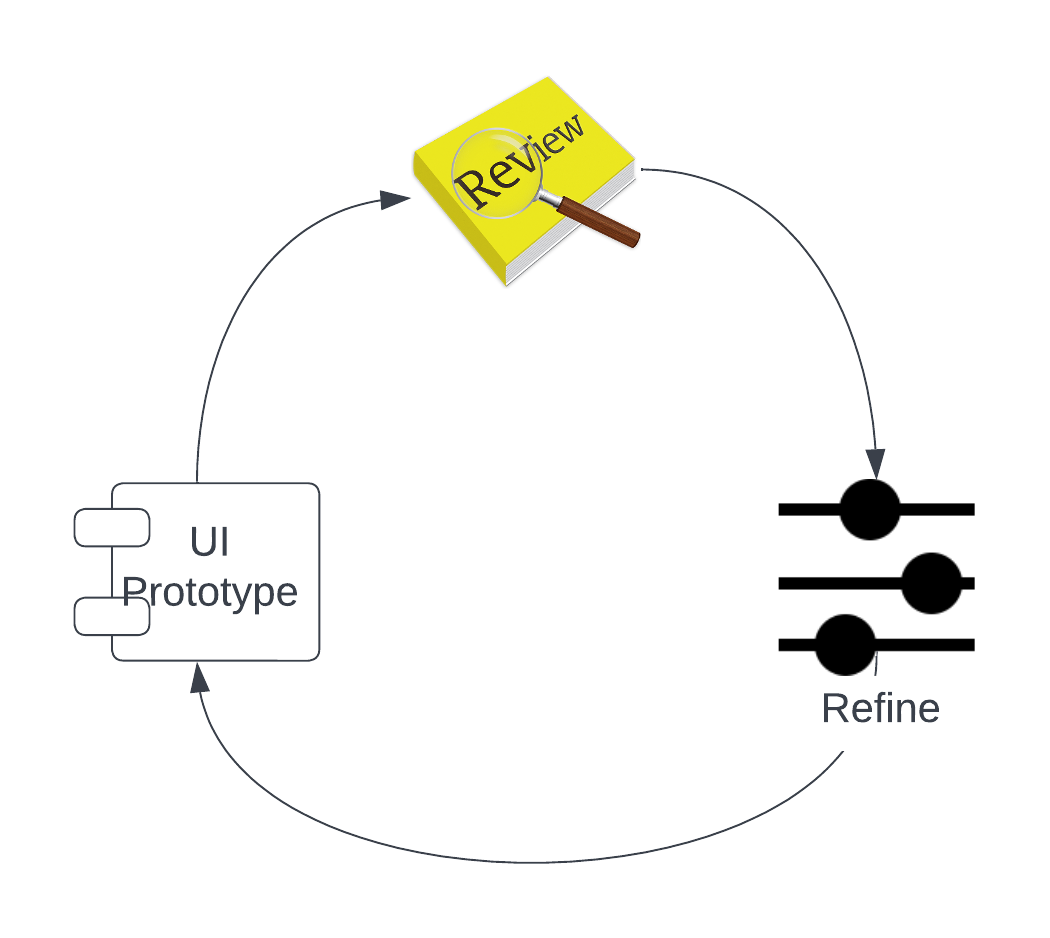
\includegraphics[width=0.6\textwidth]{PrototypingSteps.png}
  \caption[Steps of Prototyping]{Prototyping steps for an iterative development}
  \label{fig:background:stepsPrototyping}
\end{figure}
User Interface (UI) prototyping is an evaluation and testing technique according to User-Centred Design (UCD) methodology since the 1990s \cite{article:prototyping:preece}.
A UI prototype is a mock-up of the User interface.
Before a real product is created, prototypes are used to test the usability and user experience of the interface.
The evaluation of prototypes by users is a fundamental part of all iterative approaches for IT project management, especially agile methodologies \cite{article:prototyping:schwaber}.
And to build an exemplary user interface, iterative refinement must be used: develop a preliminary version of the user interface, test it with people, and make as many revisions as possible \cite{article:prototyping:gould}.
Figure \ref{fig:background:stepsPrototyping} shows a cycle that can be used for the iterative development of prototypes.
The designers start the process by developing the UI prototypes which are reviewed by different stakeholders (e.g., customers, product manager) and from the feedback received the UI prototypes are refined and the cycle is reiterated.
Therefore, designing UI prototypes enables designers and stakeholders to communicate more effectively.

An interactive prototype helps visualize design concepts and communicate new requirements and expectations about a prospective system.
Iterative design requires multiple updates to the design's execution.
\begin{figure}[htbp!]
  \centering
  \begin{subfigure}[b]{0.6\textwidth}
    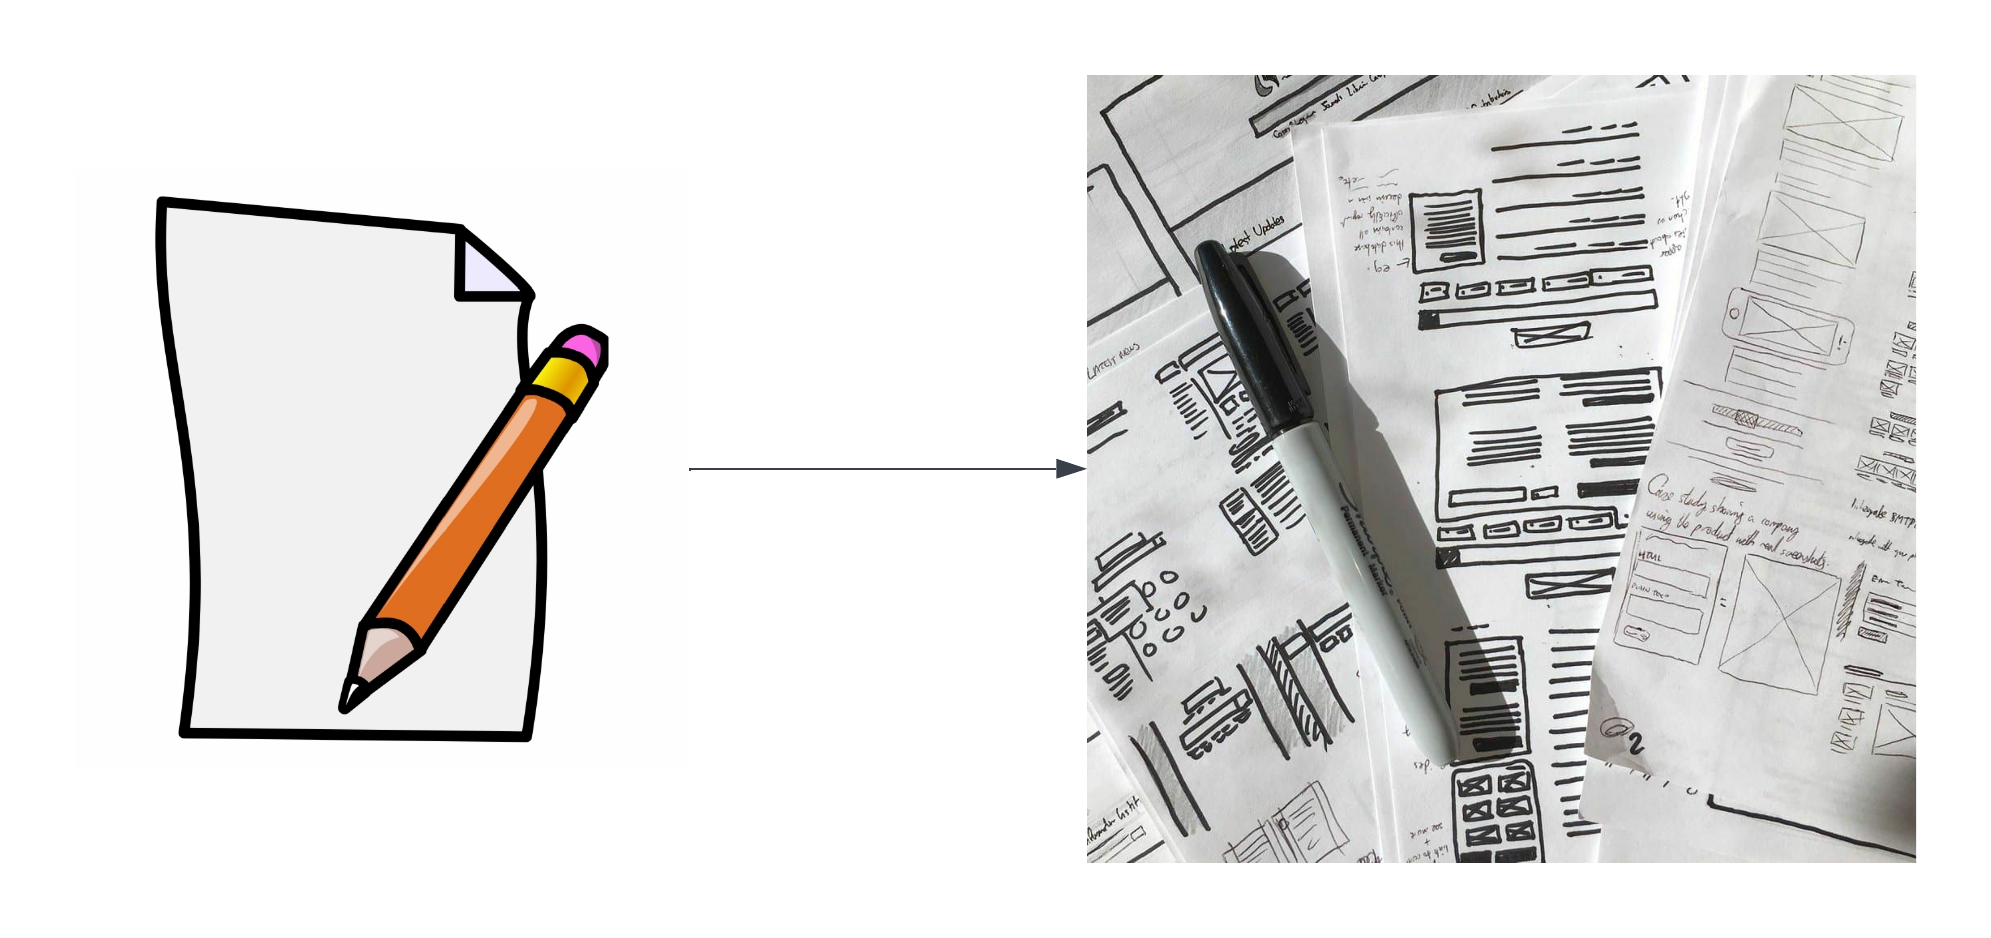
\includegraphics[width=\textwidth]{paperprototyping.png}
    \caption{Sketces and whiteboard for prototyping in initial stages of development}
    \label{fig:background:paperPrototyping}   
  \end{subfigure}             
  \begin{subfigure}[b]{0.5\textwidth}
    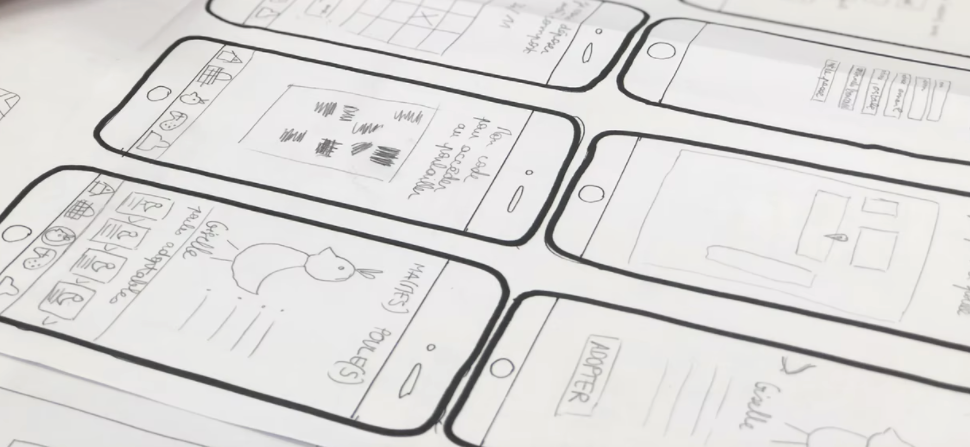
\includegraphics[width=\textwidth]{paperstepsprototypes.png}
    \caption[Paper based prototypes]{Example on how the paper-based prototypes are developed  \cite{misc:prototyping:uxpin}}
    \label{fig:background:paperprototypes}
  \end{subfigure}             
  \caption[Low fidelity prototyping]{Low fidelity prototyping}
  \label{fig:background:main}
\end{figure}
Since developing and updating the entire software system is complex and expensive, prototyping is a crucial technique \cite{article:prototyping:szekely}.
Simultaneously, software prototypes might exclude many requirements, making the software more accessible, smaller, and less expensive to construct and change \cite{article:prototyping:szekely}. 
Similarly, usability testing to validate user requirements and prototype functionality is part of the evaluation process for UI prototypes.
When prototyping is used, there is usually more contact between the designers and users, resulting in fewer usability flaws and corrections at the end of development.
The main difference between a prototype and a software application is that in a prototype the displays are designed images with no additional capabilities to display the design and flow whereas, in a software application the mockups are converted into real UI elements and a flow is available.

From a paper to HTML code, everything could be a prototype.
Jim Rudd et al. \cite{article:prototyping:highlowfidelity} have compared high and low-fidelity prototyping, explaining the advantages and disadvantages.
\textit{Low-fidelity} prototypes (see figure \ref{fig:background:paperPrototyping}) are usually limited functions, with little interaction prototyping effort. They mainly focus on explaining concepts, design alternatives, and screen layouts. 
Storyboard presentations, cards, and proof of concept prototypes come under this category.
UI designers use simple text, lines, and forms to hand-draw concepts. 
Instead of aesthetics, the focus is on speed and a ton of ideas.
To simulate user flows (as shown by figure \ref{fig:background:paperprototypes}), designers lay paper screens on the floor, table, or pinned to a board.
These prototypes emphasize communicating, educating, and informing rather than training, testing, and codification.
The advantages of low-fidelity prototypes are rapid development, lower development cost, addressing issues, and usefulness for a proof-of-concept.
Similarly, the disadvantages include limited error checking, difficulty with usability testing, navigation, flow limitation, etc.
\begin{figure}[htbp!]
  \centering    
  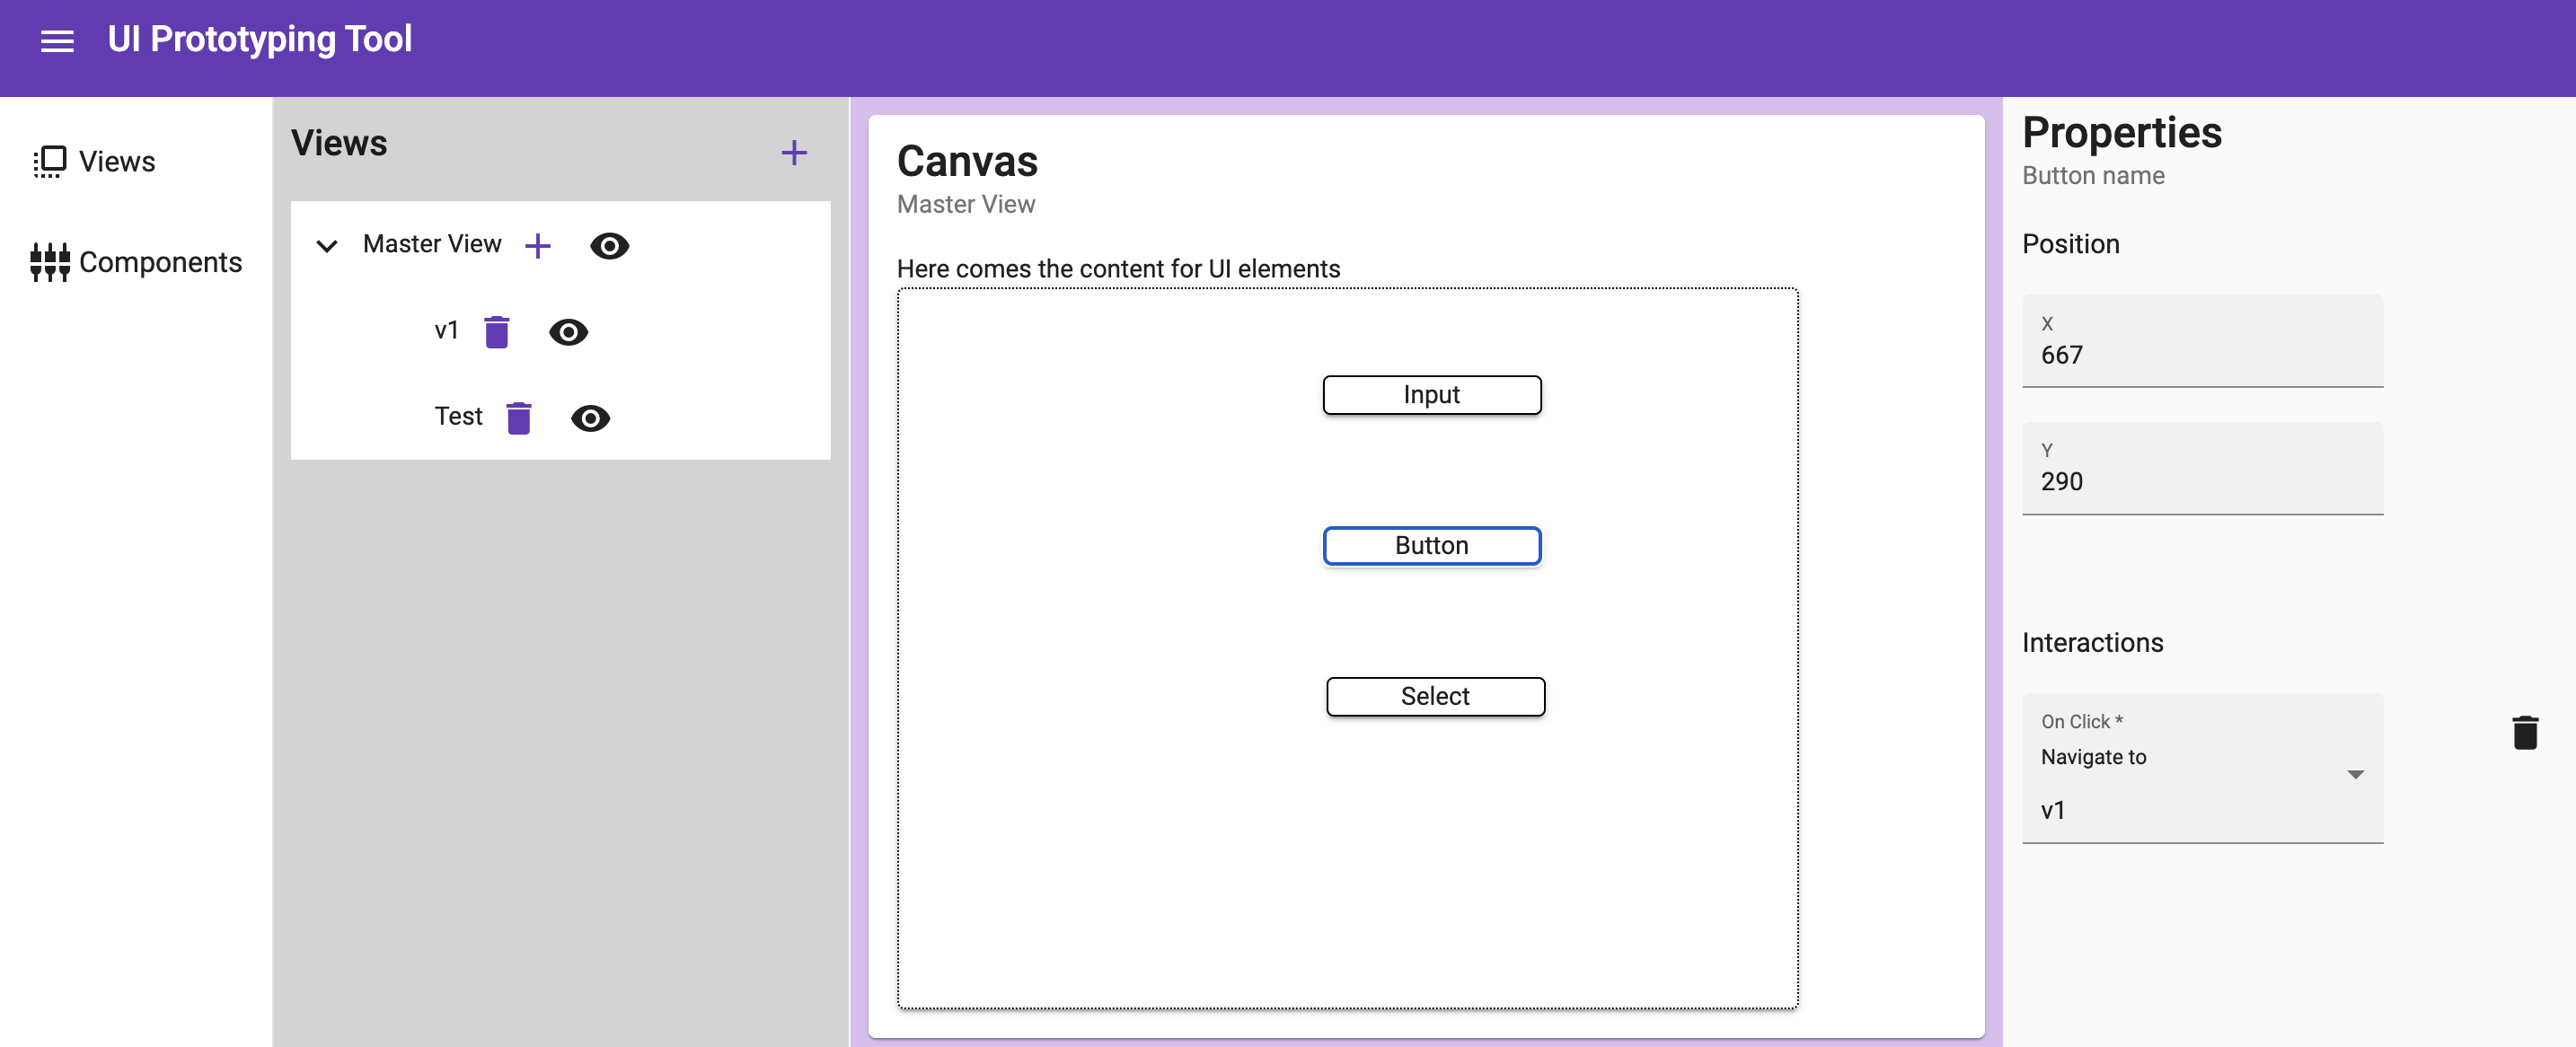
\includegraphics[width=0.9\textwidth]{ui-based-prototyping.png}
  \caption[High Fidelity prototyping]{High Fidelity prototype: Model-based UI Prototyping}
  \label{fig:background:uiPrototyping}
\end{figure}

Contrary to low-fidelity prototypes, \textit{High-fidelity} prototypes (see figure \ref{fig:background:uiPrototyping}) have full functionality and focus on flow, and the user models of the system \cite{article:prototyping:exploratory}.
The users can operate these prototypes, and the developers can collect information from the users through measurements. 
Other advantages of high-fidelity prototypes are that they are user-driven, used for navigation and tests, and can also be served as a marketing tool for attracting potential customers \cite{article:prototyping:highlowfidelity}.\\ \\
\textit{Steps for creating UI Prototypes}:
\begin{itemize}
  \item \textbf{Learn about your consumers' requirements:} Here, our primary goal is to understand the principles that underlie our client's values to better our service to suit their needs. In this step, the design team meets with the product management team and brainstorms to develop some use cases and end-user needs. After the discussions, the team can present the customers to make sure they are on the right track and the design matches their requirements.
  \item \textbf{Sketch out the product:} This is an important step for UI designers. In this step, Low fidelity prototypes can be developed e.g., The design team can create the paper prototypes and start brainstorming on different possible options. Further, the team can create high-fidelity prototypes by using some tools. There are some tools available like Figma\footnote{Figma: \url{https://www.figma.com/}}, Invision\footnote{Invion AG \url{https://www.invisionapp.com/}}, Adobe XD\footnote{Adobe XD: \url{https://www.adobe.com/products/xd.html}}, Axure RP\footnote{Axure RP: \url{https://www.axure.com/}} and many more. Using these tools, the designer can develop some high-fidelity digital prototypes.
  \item \textbf{Develop into Software:} This step includes the software developers and the designers coordinating and developing the software in iterations. The designers would give feedback to the software developers and they would be continuously developing the product.
\end{itemize}

After performing these steps, it is necessary to test if everything is working as expected by the user requirements.
It is necessary to make sure that the product is usable for the end-users and that developers do not miss any important features.
This can be performed in the evaluation phase. 

%********************************** % Low code **************************************
\section{Low Code / No Code Development Platform}
\label{background:section:lowcode}
Low Code is a technique used by developers to help non-developers design and develop software applications using a \textit{Graphical User Interface} (GUI) supported by a \textit{Low Code Development Platform} (LCDP).
Similarly, there is another technique called no code supported by the \textit{No Code Development Platform} (NCDP) \cite{article:nocode:miller}.
Unlike low code, no-code platforms require no programming skills because they offer some prebuild templates for building the apps.
Using the visual user interface and ready-made automatic tools on these application development platforms, it is feasible to create apps relatively quickly. 
These technologies are visual app development methods that speed up app creation by using drag-and-drop editors and pre-built components. 
By allowing software developers to concentrate on challenging coding areas, low code / no code accelerates platform development.
Due to its simplicity, flexibility and low cost, companies have started using this platform to meet the high demands of software development and digitalization.
Low code is a software development method that uses less human coding to enable users to construct and manage programs efficiently \cite{article:nocode:sahina}.
Additionally, it lowers the expenses associated with initial installation, training, distribution, and maintenance \cite{article:nocode:sanchi}.\\ \\
\textit{Main Steps Of \textbf{Low-Code} App Development}
\paragraph*{Building:}
\begin{figure}[htbp!]
  \centering    
  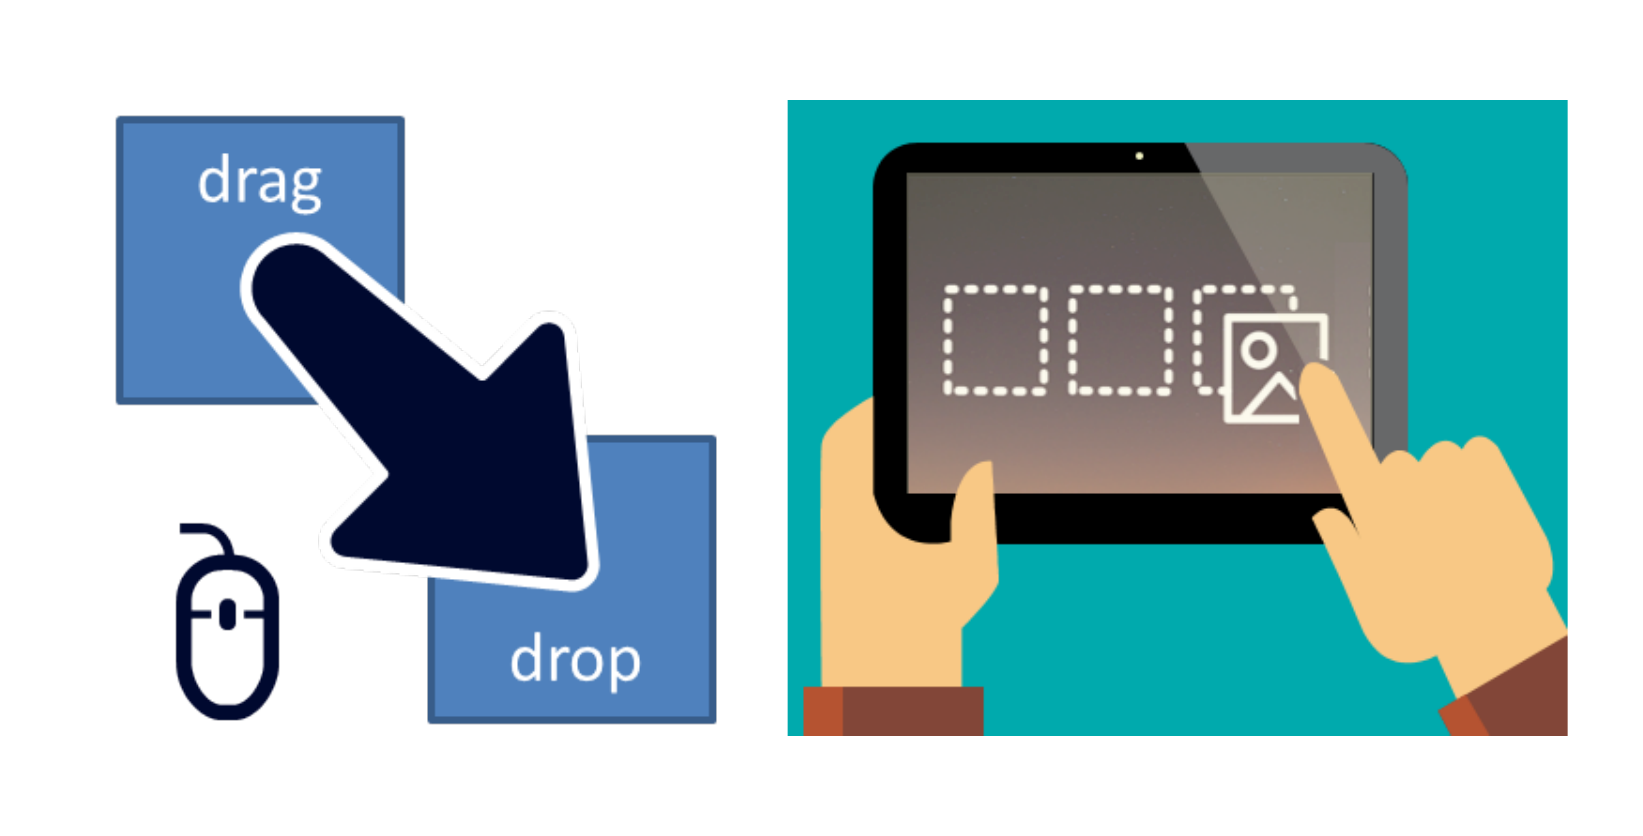
\includegraphics[width=0.7\textwidth]{step1-building.png}
  \caption[Building]{Step 1: Building of Low Code App development}
  \label{fig:background:building}
\end{figure}
In this step (as shown in the figure \ref{fig:background:building}), the platform gives you the freedom to alter the provided code and add hand-written custom code to it to specify more complex features in the app as you create the app step-by-step using visual editors and drag and drop interfaces.
Modules, components, and chart-builders are already incorporated into low-code applications. 
Charts may be used to display data from modules, while modules are used to specify the type of data that will be stored in the app. 
Components and pages provide the type of user experience the app will have.
These platforms also have a provision for the automation of repetitive tasks in the app.
\paragraph*{Testing:}
\begin{figure}[htbp!]
  \centering    
  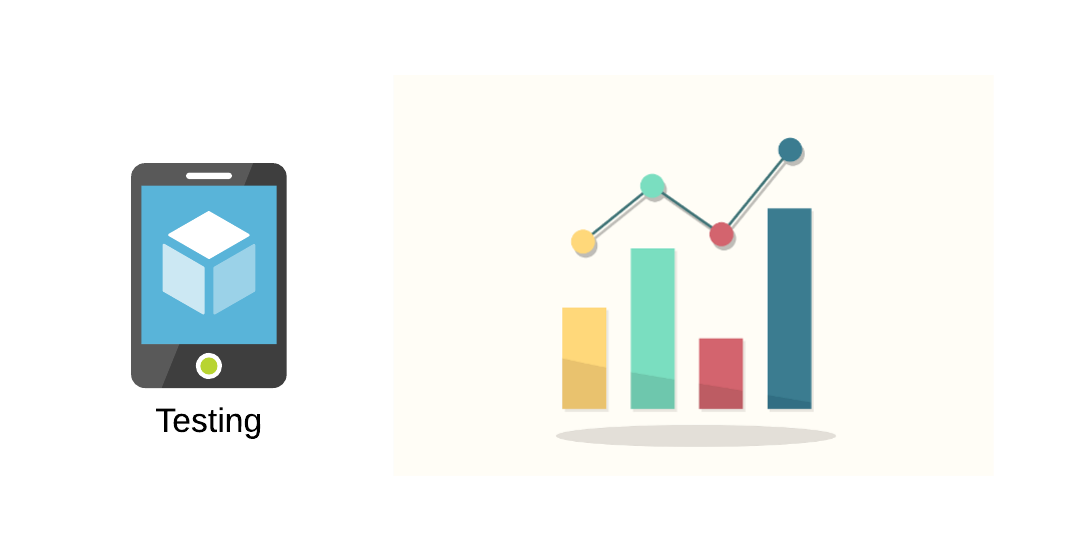
\includegraphics[width=0.9\textwidth]{step2-testing.png}
  \caption[Testing]{Step 2: Testing of Low Code App development}
  \label{fig:background:testing}
\end{figure}
Testing a software application is an important part of the development cycle.
However, the low-code development platform decreases the requirement for testing. 
Pre-build modules and components on low-code platforms are created with a certain level of application security. 
The developers of the low-code platform constantly monitor these modules, and they have previously gone through several unit tests.
But (as shown in figure \ref{fig:background:testing}), we still do need to perform the test on the entire application after integration for scrutiny and this is performed in this step.
\paragraph*{Deploying:}
\begin{figure}[htbp!]
  \centering    
  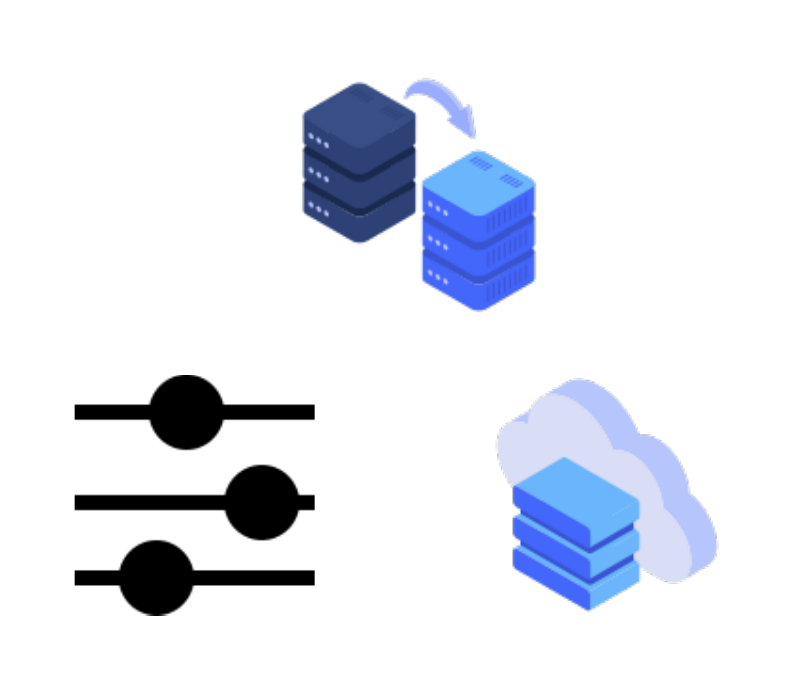
\includegraphics[width=0.7\textwidth]{step3-deployment.png}
  \caption[Testing]{Step 3: Deployment of Low Code App development}
  \label{fig:background:deploying}
\end{figure}
In this step, the application is deployed across apps and to the final users.
In LCDP, the packages for installation, configurations, and application setup are included.
And, the deployment of the app can be done on various services (see figure \ref{fig:background:deploying}) like Cloud-based services.
This means that the LCDP gives freedom to the users in deploying the applications for the customers with just one click.  \\\\
\textit{Some features that make the LCDP or NCDP favorable for development} \cite{article:nocode:sahina, article:nocode:ihirwe, paper:lowcode:cabot}
\begin{itemize}
  \item \textbf{Re-usable components:} LCDP usually contains pre-configured components, modules, logic, templates, and many more that can be customized as per customer requirements. This helps to Build apps with consistency and scalability. Also, the scope for testing decreases as the components of the LCDP is pre-tested for security and performance. 
  \item \textbf{Flexible and Model-driven development:} The drag-and-drop functionality helps developers increase their productivity whereas for citizen developers to build all types of apps. LCDP ensures to have a GUI useful for the non-developers. Therefore, it encourages the stakeholders outside the IT department to participate in development. Low code has become famous in model-driven development. Model-driven development helps to visualize how the app works while it is built.
  \item \textbf{Easy deployment:} This feature ensures that the artifacts are created and the platform is ready to deploy. LCDP has packages that contain various deployment packages (e.g., \texttt{Dockerfile} to deploy on docker\footnote{Docker: \url{https://www.docker.com/}})
\end{itemize}

Additionally, a variety of options are provided for developers with little programming experience, those with coding expertise and seasoned programmers who wish to expand the functionality of the current design \cite{article:nocode:sahina}.

%********************************** % Model-Based Software Engineering **************************************
\section{Model-based Software Engineering}
\label{background:section:mbse}
\begin{figure}[htbp!]
  \centering    
  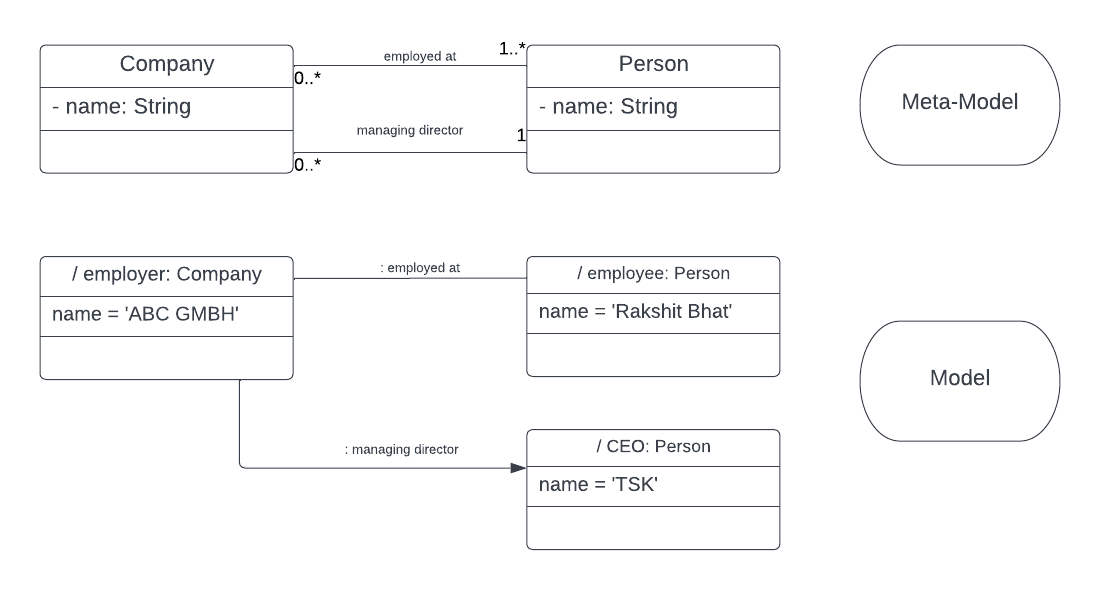
\includegraphics[width=0.9\textwidth]{meta-models.png}
  \caption[Meta models]{Meta models and Models}
  \label{fig:background:m1m2}
\end{figure}

Model-based Software Engineering (MBSE) refers to maintaining and developing software while reusing existing code.
Similarly, Model-driven software engineering (MDSE) is the term used to cover various techniques for creating software using codified models.
The development of domain-specific languages (DSLs) is becoming essential in language engineering due to the growth in model-driven engineering (MDE) \cite{article:mbse:cuadrado}.
At the same time, for creating models, the Model Object Facility (MOF) has defined three levels separating the reality, models, meta-models and meta-meta-models (as shown in the figure \ref{fig:background:moflevels}).
\begin{figure}[htbp!]
  \centering    
  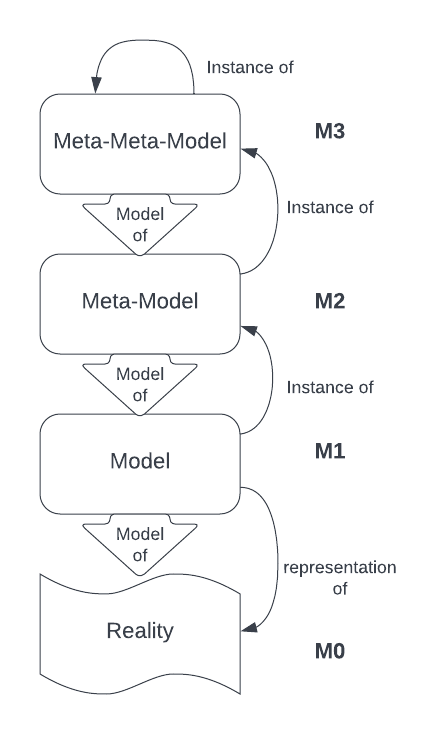
\includegraphics[width=0.5\textwidth]{mof-meta-modelling.png}
  \caption[MOF levels]{Model Object Facility (MOF) levels}
  \label{fig:background:moflevels}
\end{figure}
\paragraph{Meta Models:} Meta-model is defined as a model of a model or a simplified version of an actual model of a system of interest or a software application.
Meta models can act as an intermediary between the input and the output relations and can represent mathematical relations or algorithms.
A model is usually defined as an abstraction of real-world entities, and a metamodel is another abstraction of the models. 
Similarly, metamodelling is a process of analysis and development of the rules, theories and models useful for constructing meta-models.
From figure \ref{fig:background:m1m2}, the meta-models are very similar to the UML class diagrams and the models are instances of them. 

Adaptive model-driven user interface development systems are developed \cite{article:mbse:akiki}.
In this research, the authors defined twenty properties challenges for the Model-driven User interface and compared some tools that implement these properties.

Companies use different modeling languages to codify the UIs.
Cameleon \cite{article:cameleon:balme} is a framework that divides the UI into several elements to maximize the parts' reusability in various user, platform, and environment situations.
A platform-independent abstract UI, a platform-dependent concrete UI, and a device-dependent final UI are the layers the framework offers to accomplish this.
A standardized modeling language for software product content, abstract UI models, user interactions, and control behavior is Interaction Flow Modeling Language (IFML) \cite{article:ifml:piero}.
As a result, IFML relies on the platform-independent display of the UI that can be utilized on several platforms and devices.

However, these modeling languages do not emphasize offering visual notations to aid non-developers in creating such interfaces. 
A recent method \cite{article:mbse:bexiga} illustrates how to use low-code approaches to close the gap between designers and developers.

%********************************** % Task-based Usability Testing **************************************
\section{Task-based Usability Testing}
\label{background:section:task}
The main focus of usability testing is that seeing someone use an interface is the best approach to determine what functions well and what doesn't. 
Assigning tasks to the accurate number of participants can help determine the quality of the UI and the problems faced by the users. 
Overall, the UI design can be improved using the participants' feedback. 
Task-based usability testing is one way to determine the software's overall usability \cite{article:usability:doesburg} by measuring the percentage of the tasks the users complete.
To observe the participants, they need to be assigned some ``activities'' or \textit{tasks}. 
These tasks need to be some scenarios, not just "\textit{do something}", because it sets the users a stage for \textit{why} they would perform the tasks. 
To get qualitative feedback from the participants, in \cite{misc:usability:tasks}, the authors provide \textit{three good practices} and task-writing tips for designing better task scenarios.
\textit{(1) Make the Task Realistic}.
So, the participants should be able to execute the tasks which could be completed efficiently and with the freedom to make their own choices.
\textit{(2) Make the Task Actionable}.
Here, the participants should be told what they need to do rather than how they would do it.
\textit{(3) Avoid Giving Clues and Describing the Steps}.
The participants should expose the navigation and some features on their own, giving accurate feedback about the interface.
The task scenario example\footnote{Task based usability: \url{https://www.nngroup.com/articles/task-scenarios-usability-testing/}} below sets a target for the participants to locate a movie from our \textit{Videostreamer} app.
\begin{itemize}
  \item[] \textbf{Good and bad example of a task scenario}
  \item \textbf{User goal:} Find a movie. 
  \item \textbf{Bad task scenario:} You should watch a movie on Sunday afternoon. Go to\\ \textit{www.videostreamer.com}, navigate to the Movies page, and find the movie as per the schedule.
  \item \textbf{Good task scenario:} Use \textit{www.videostreamer.com} to find a movie that fits your interest that you'd be interested in watching on Sunday afternoon. 
\end{itemize}
In this example, the \textit{bad} task scenario gives detailed information about the navigation, violating the third tip.
\clearpage
%********************************** % Experimentation **************************************
\section{Experimentation}
\label{background:section:experimentproduct}
Experimental Product Design (EPD) has become integral to optimizing UI and \textit{User Experience (UX)}.
Experimentation helps product teams test out ideas early in the process with real-world consumers rather than settling on a single solution and executing it in the final phase \cite{misc:CE:miklos}.
In this section, we discuss the role that experimentation plays in the software development process and how designers can ``prototype with real data'' to improve the usability of the UI.
\begin{figure}[htbp!]
  \centering    
  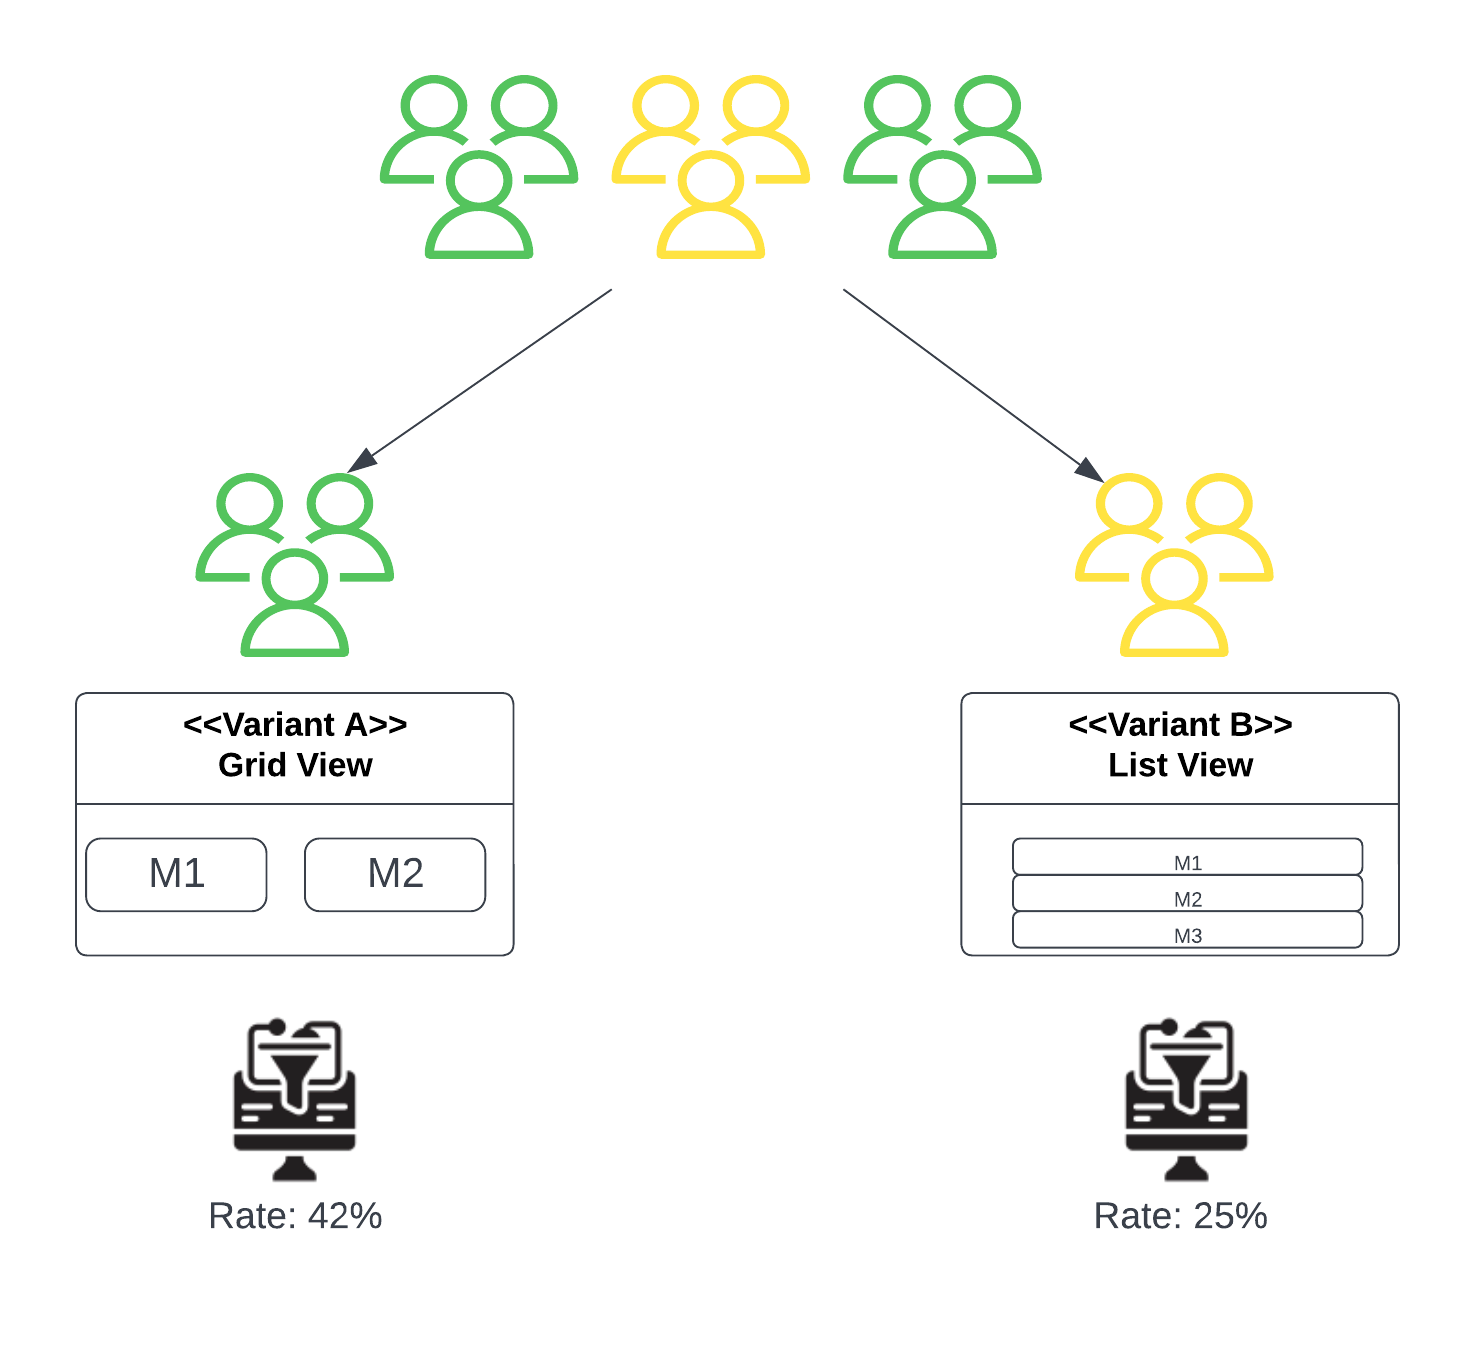
\includegraphics[width=0.5\textwidth]{ab-testing.png}
  \caption[A/B Testing]{A/B Testing}
  \label{fig:background:abtesting}
\end{figure}
For conducting experiments, various steps like \textbf{Users distribution}, \textbf{Continuous Experimentation}, \textbf{Variants distribution}, \textbf{Measurements}, and \textbf{Refining the model} exist.  

\paragraph{User distribution:} To conduct a successful experiment, the size of the study, or the number of participants, must be considered first.
Statistics suggest that the more people you include in the investigation, the greater its statistical power, which impacts your level of confidence in your findings \cite{misc:experimentation:users}.
The next step is to allocate the participants to treatment groups at random. 
There are several levels of treatment given to each group (e.g., some prerequisites to the participants before experimenting).
For assigning the subjects to groups, users are divided into a \textit{between-subjects design} vs a \textit{within-subjects design}.
In a between-subjects design, individuals receive only one of the possible levels of an experimental treatment whereas, in a within-subjects design, every individual receives each of the experimental treatments consecutively, and their responses to each treatment are measured.
In figure \ref{fig:background:abtesting}, a between-subject design is used where only one of the variants is assigned to the user.

\paragraph{Continuous Experimentation and Variants distribution:} 
Continuous experimentation (CE) primarily aims to get users' feedback on the software product's evolution.
As per figure \ref{fig:background:abtesting}, CE generally uses A/B/n testing in a primary case of comparing two variants, A and B, which are controlled and test variables in an experiment.
First, the users or the participants of the study are separated into groups and are assigned one of the two variants.
Since we have \texttt{GridView} and the \texttt{ListView}, one group of the users are assigned with List and one with Grid View (see figure \ref{fig:background:abtesting}).
Then both users would be given some tasks (see Section \ref{background:section:task}), and the analysis of these tasks gives the winner among the variants.  
And in the end, developers make evidence-based decisions to direct the progress of their software by continuously measuring the results of multiple variants performed in an experimental context with actual users \cite{article:CE:ros}.
CE is an extension to the introduction of continuous integration and deployment, and all are summarized as constant software engineering \cite{article:CE:fitzgerald}.

\paragraph{Examples of A/B Testing:}
Some tools conduct A/B Testing and are used to improve User Interface. \textit{Optimizely}\footnote{Optimizely: \url{https://www.optimizely.com/}}, \textit{Adobe Target}\footnote{Adobe Target: \url{https://business.adobe.com/in/products/target/adobe-target.html}}, \textit{Petri}\footnote{Petri: \url{https://github.com/wix-incubator/petri}}, \textit{Google Analytics and Google Optimize}\footnote{Google Analytics and Google Optimize: \url{https://vwo.com/compare/google-optimize/}} are some of the research tools which can be used to conduct A/B Testing.

\clearpage

% \begin{landscape}

% \section{Landscape}
% I can cite Wall-E (see Fig.~\ref{fig:WallE}) and Minions in despicable me (Fig.~\ref{fig:Minnion}) or I can cite the whole figure as Fig.~\ref{fig:animations}


% \begin{figure}
%   \centering
%   \begin{subfigure}[b]{0.3\textwidth}
%     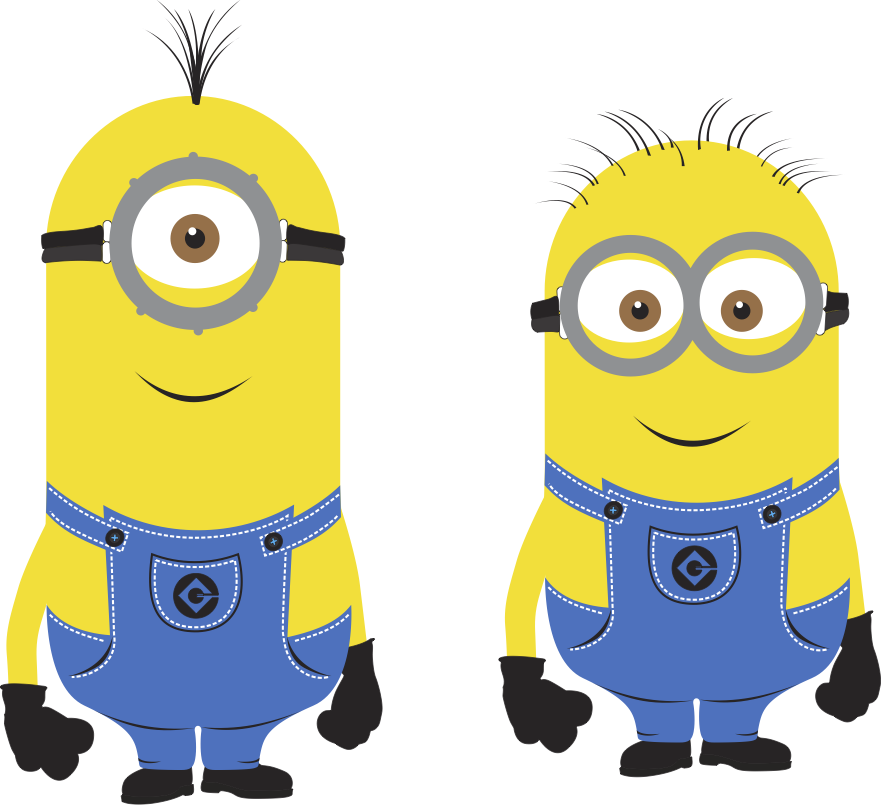
\includegraphics[width=\textwidth]{minion.png}
%     \caption{Tom and Jerry}
%     \label{fig:TomJerry}   
%   \end{subfigure}             
%   \begin{subfigure}[b]{0.3\textwidth}
%     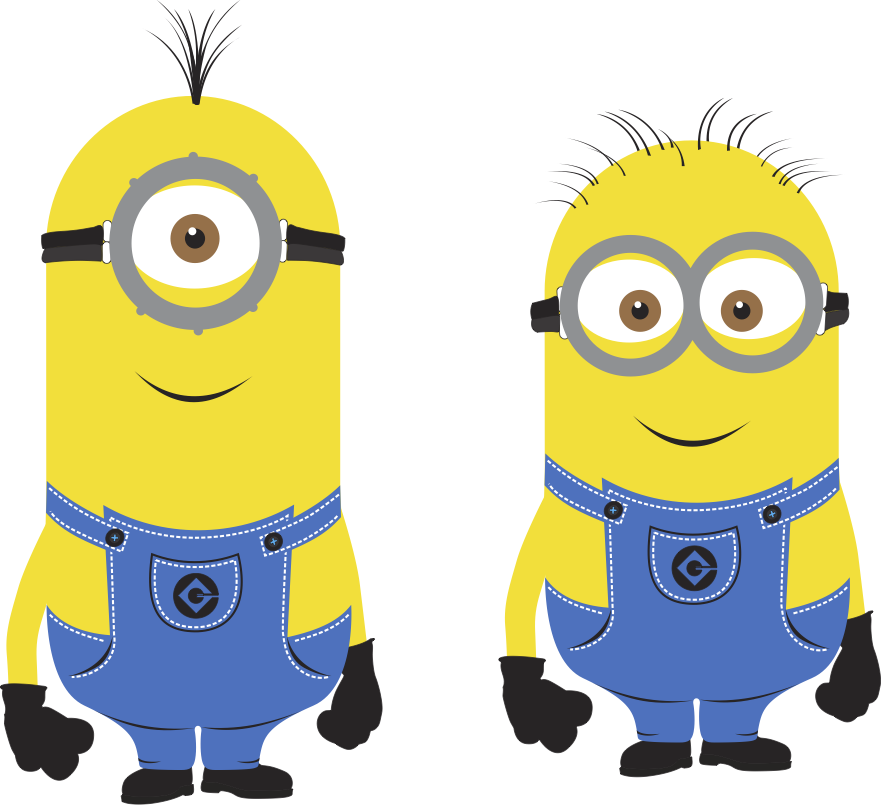
\includegraphics[width=\textwidth]{minion.png}
%     \caption{Wall-E}
%     \label{fig:WallE}
%   \end{subfigure}             
%   \begin{subfigure}[b]{0.3\textwidth}
%     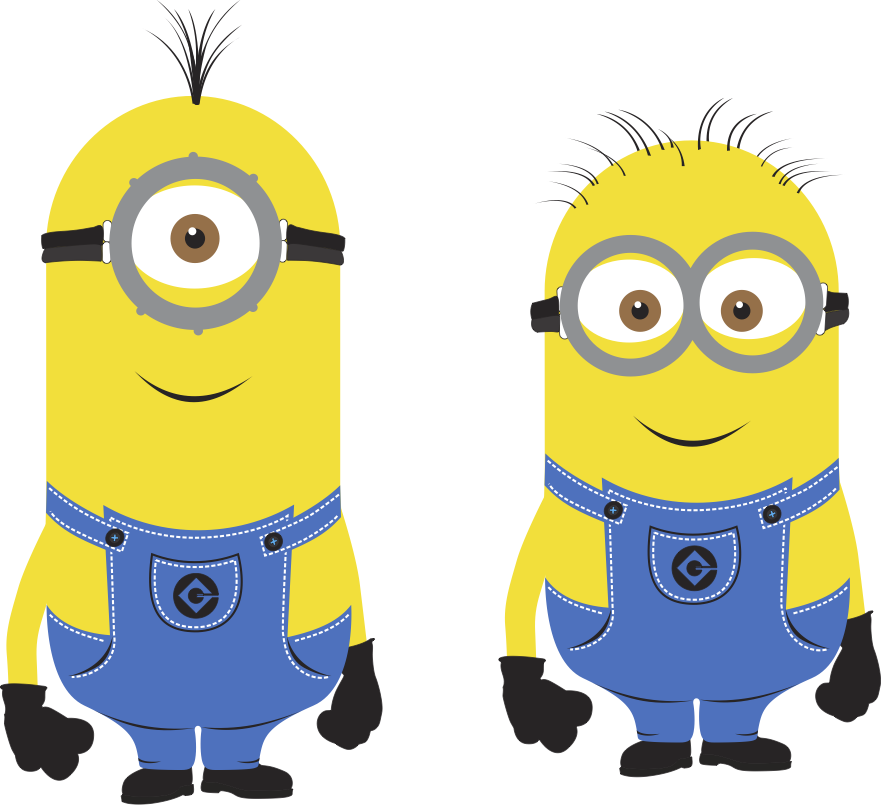
\includegraphics[width=\textwidth]{minion}
%     \caption{Minions}
%     \label{fig:Minnion}
%   \end{subfigure}
%   \caption{Best Animations}
%   \label{fig:animations}
% \end{figure}

% \end{landscape}
